\chapter[Baterias]{Baterias Automotivas}

As baterias dos automóveis possuem normalmente essa força eletromotriz de 12 V, pois são compostas de 6 pilhas ou células de chumbo-ácido. E elas são também denominadas como baterias de chumbo, porque o seu ânodo (polo negativo) são as placas de chumbo e o seu cátodo (polo positivo) são as placas de chumbo com óxido e chumbo IV ($\mathrm{Pb O_2}$).
Essas baterias possuem altas correntes, que permitem dar partida em motores graças aos elevados valores de densidade de potência que apresentam.
Como se observa na figura abaixo, as placas de chumbo revestidas de $\mathrm{Pb O_2}$ (placas negativas) são ligadas ao conector positivo. Enquanto que as placas de chumbo (placas positivas) são ligadas ao conector negativo. Elas são separadas por algum papelão, plástico ou algum papel separador microporoso.
Esse conjunto é colocado no compartimento da bateria e mergulhadas em uma solução aquosa de ácido sulfúrico ($\mathrm{H_2 SO_4}$) com uma densidade de aproximadamente $1,28 g/cm^{3}$	.

\begin{figure}[h]
  \centering
  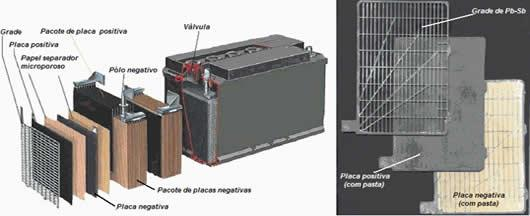
\includegraphics[width=400px, scale=1]{figuras/bateria}
  \caption{Bateria com placa de chumbo}
\end{figure}

As semirreações e a reação global que ocorrem nessa bateria são:\\
Ânodo: $\mathrm{Pb}$ + $\mathrm{HSO_4^{1-}}$ + $\mathrm{H_2 O}$ $\leftrightarrow$ $\mathrm{PbSO_4}$ + $\mathrm{H_3 O^{1+}}$ + 2e-\\
Cátodo: $\mathrm{Pb O_2}$ + $\mathrm{HSO_4^{1-}}$ + $\mathrm{3 H_3 O^{1+}}$ + 2e- $\leftrightarrow$ $\mathrm{PbSO_4}$ + $\mathrm{5 H_2 O}$\\
\dotfill\\
Reação global: $\mathrm{Pb}$ + $\mathrm{PbO_2}$ + $\mathrm{2HSO_4^{1-}}$ + $\mathrm{2H_3 O^{1+}}$ $\leftrightarrow$ $\mathrm{2PbSO_4}$ + $\mathrm{4 H_2 O}$

Como pode ser observado pela seta dupla acima, essas reações são reversíveis, o que significa que é possível recarregar novamente as baterias de chumbo por se fornecer energia ao sistema, ou seja, é possível passar uma corrente elétrica fornecida por um gerador de corrente contínua. Desse modo, o sentido dessas reações é invertido, ocorrendo a regeneração de grande parte do ácido sulfúrico e carregando, assim, a bateria. No automóvel, essa diferença de potencial que fornece energia e recarrega a bateria é feita pelo dínamo ou pelo alternador.
A densidade do ácido sulfúrico ajuda a identificar se a bateria está decarregada. Visto que sua densidade é 1,28g/cm3; se este valor estiver abaixo de 1,20 g/cm3, significa que o ácido sulfúrico foi consumido e a bateria está descarregada. Por isso, essas baterias são muito duráveis.
